\section{研究背景}
%TODO:伸縮センサのお話を書く
soft robotics toolkit\cite{MITSoftRobot}において,シリコンと導電性布をもちいた伸縮センサが紹介されていた.本センサは,伸縮性に優れており,柔軟性も兼ね備えたものとなっている.また,製作コストも\$23と非常に安価なものであると紹介されている.
\begin{figure}[h]
    \begin{center}
        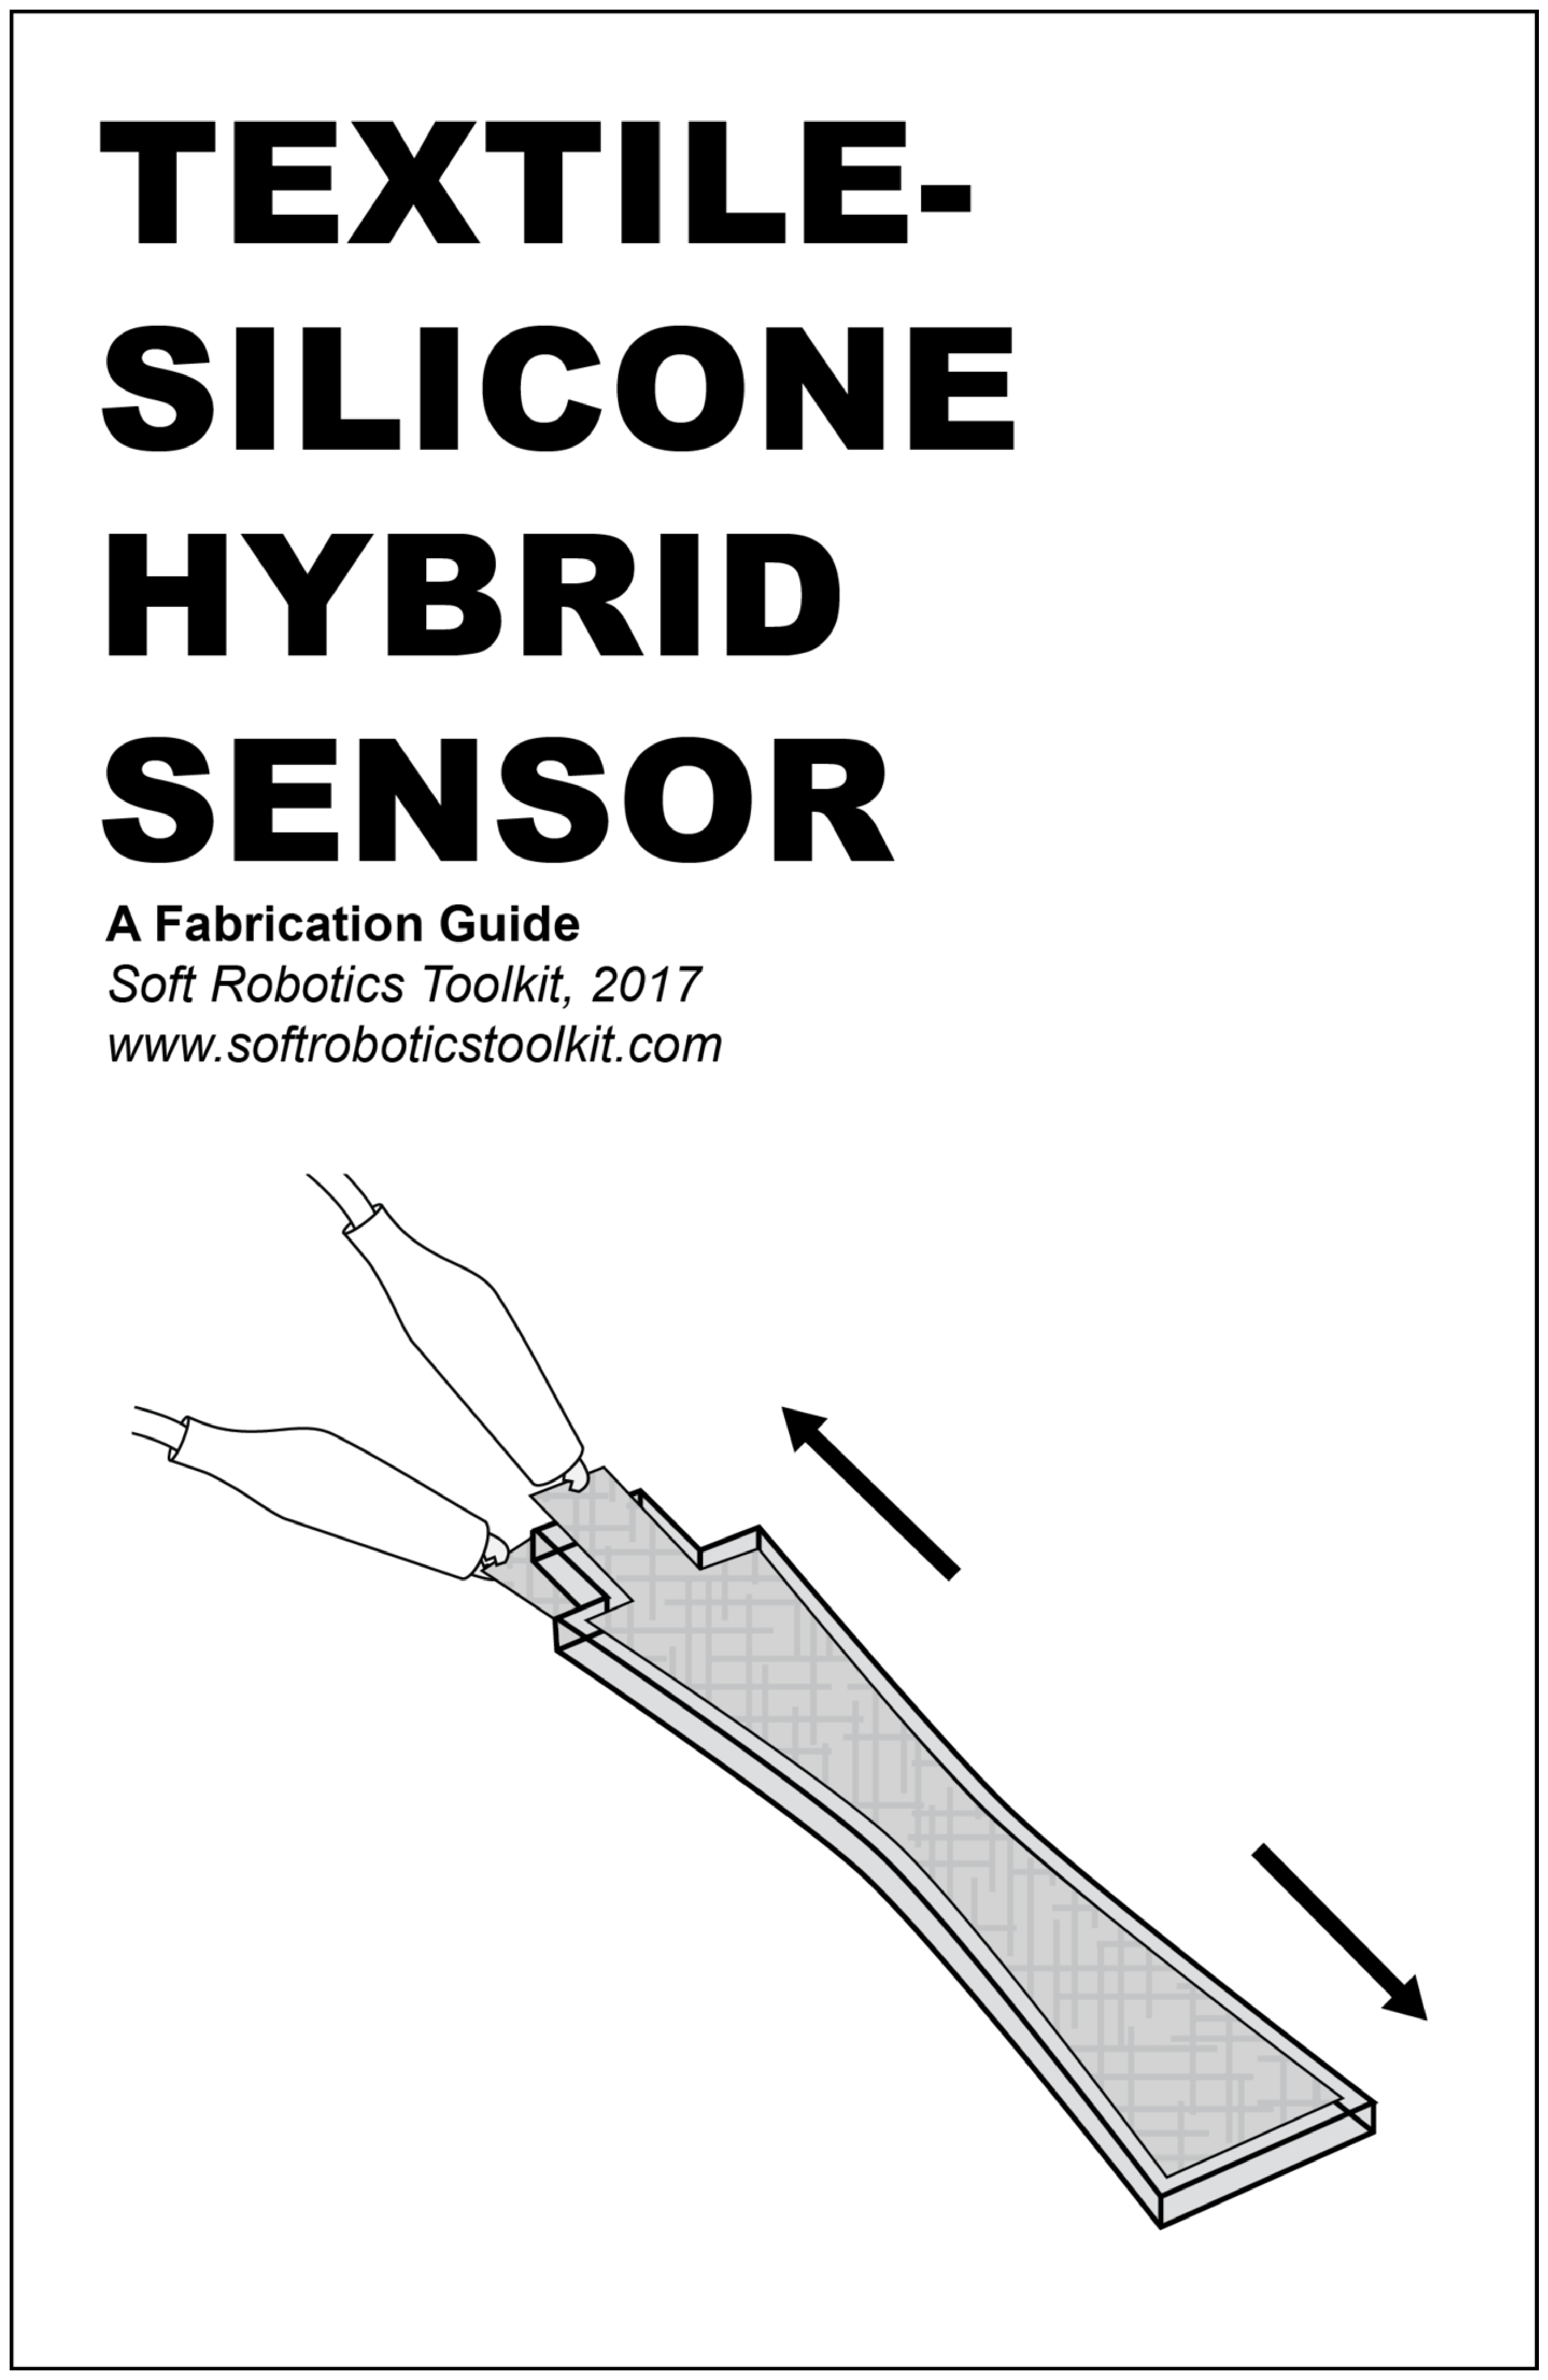
\includegraphics[width=0.5\columnwidth,clip]{Photo/BackGround/MITSoftRobotics.eps}
        \caption{soft roboticstool kit 表紙\cite{MITSoftRobot}}
        \label{MITSoftRobot表紙}
    \end{center}
\end{figure}

%TODO:初号機体のお話を書く
%TODO:初号機関連の研究のリファレンスを貼る
当研究室において先行研究として,人間の筋肉を模した空気圧人工筋をもちいたペダリングロボット(初号機)が存在する.これは,人間のペダリング動作における筋シナジーの計測を行い,ロボットに再現させるものであった.筋シナジーの計測は片麻痺患者,健常者ともに行い,片麻痺患者におけるペダリング動作時の特徴的な活動状態を健常者との比較を行った.本ロボットは,腰がサドル上に固定された状態で股関節,膝関節,足首関節それぞれがピッチ方向にのみ自由度を持っており2次元平面上における動作を再現することが出来た.また本動作を再現するために空気圧人工筋を片足8筋分用いて行っていた.
\begin{figure}[h]
 \begin{center}
  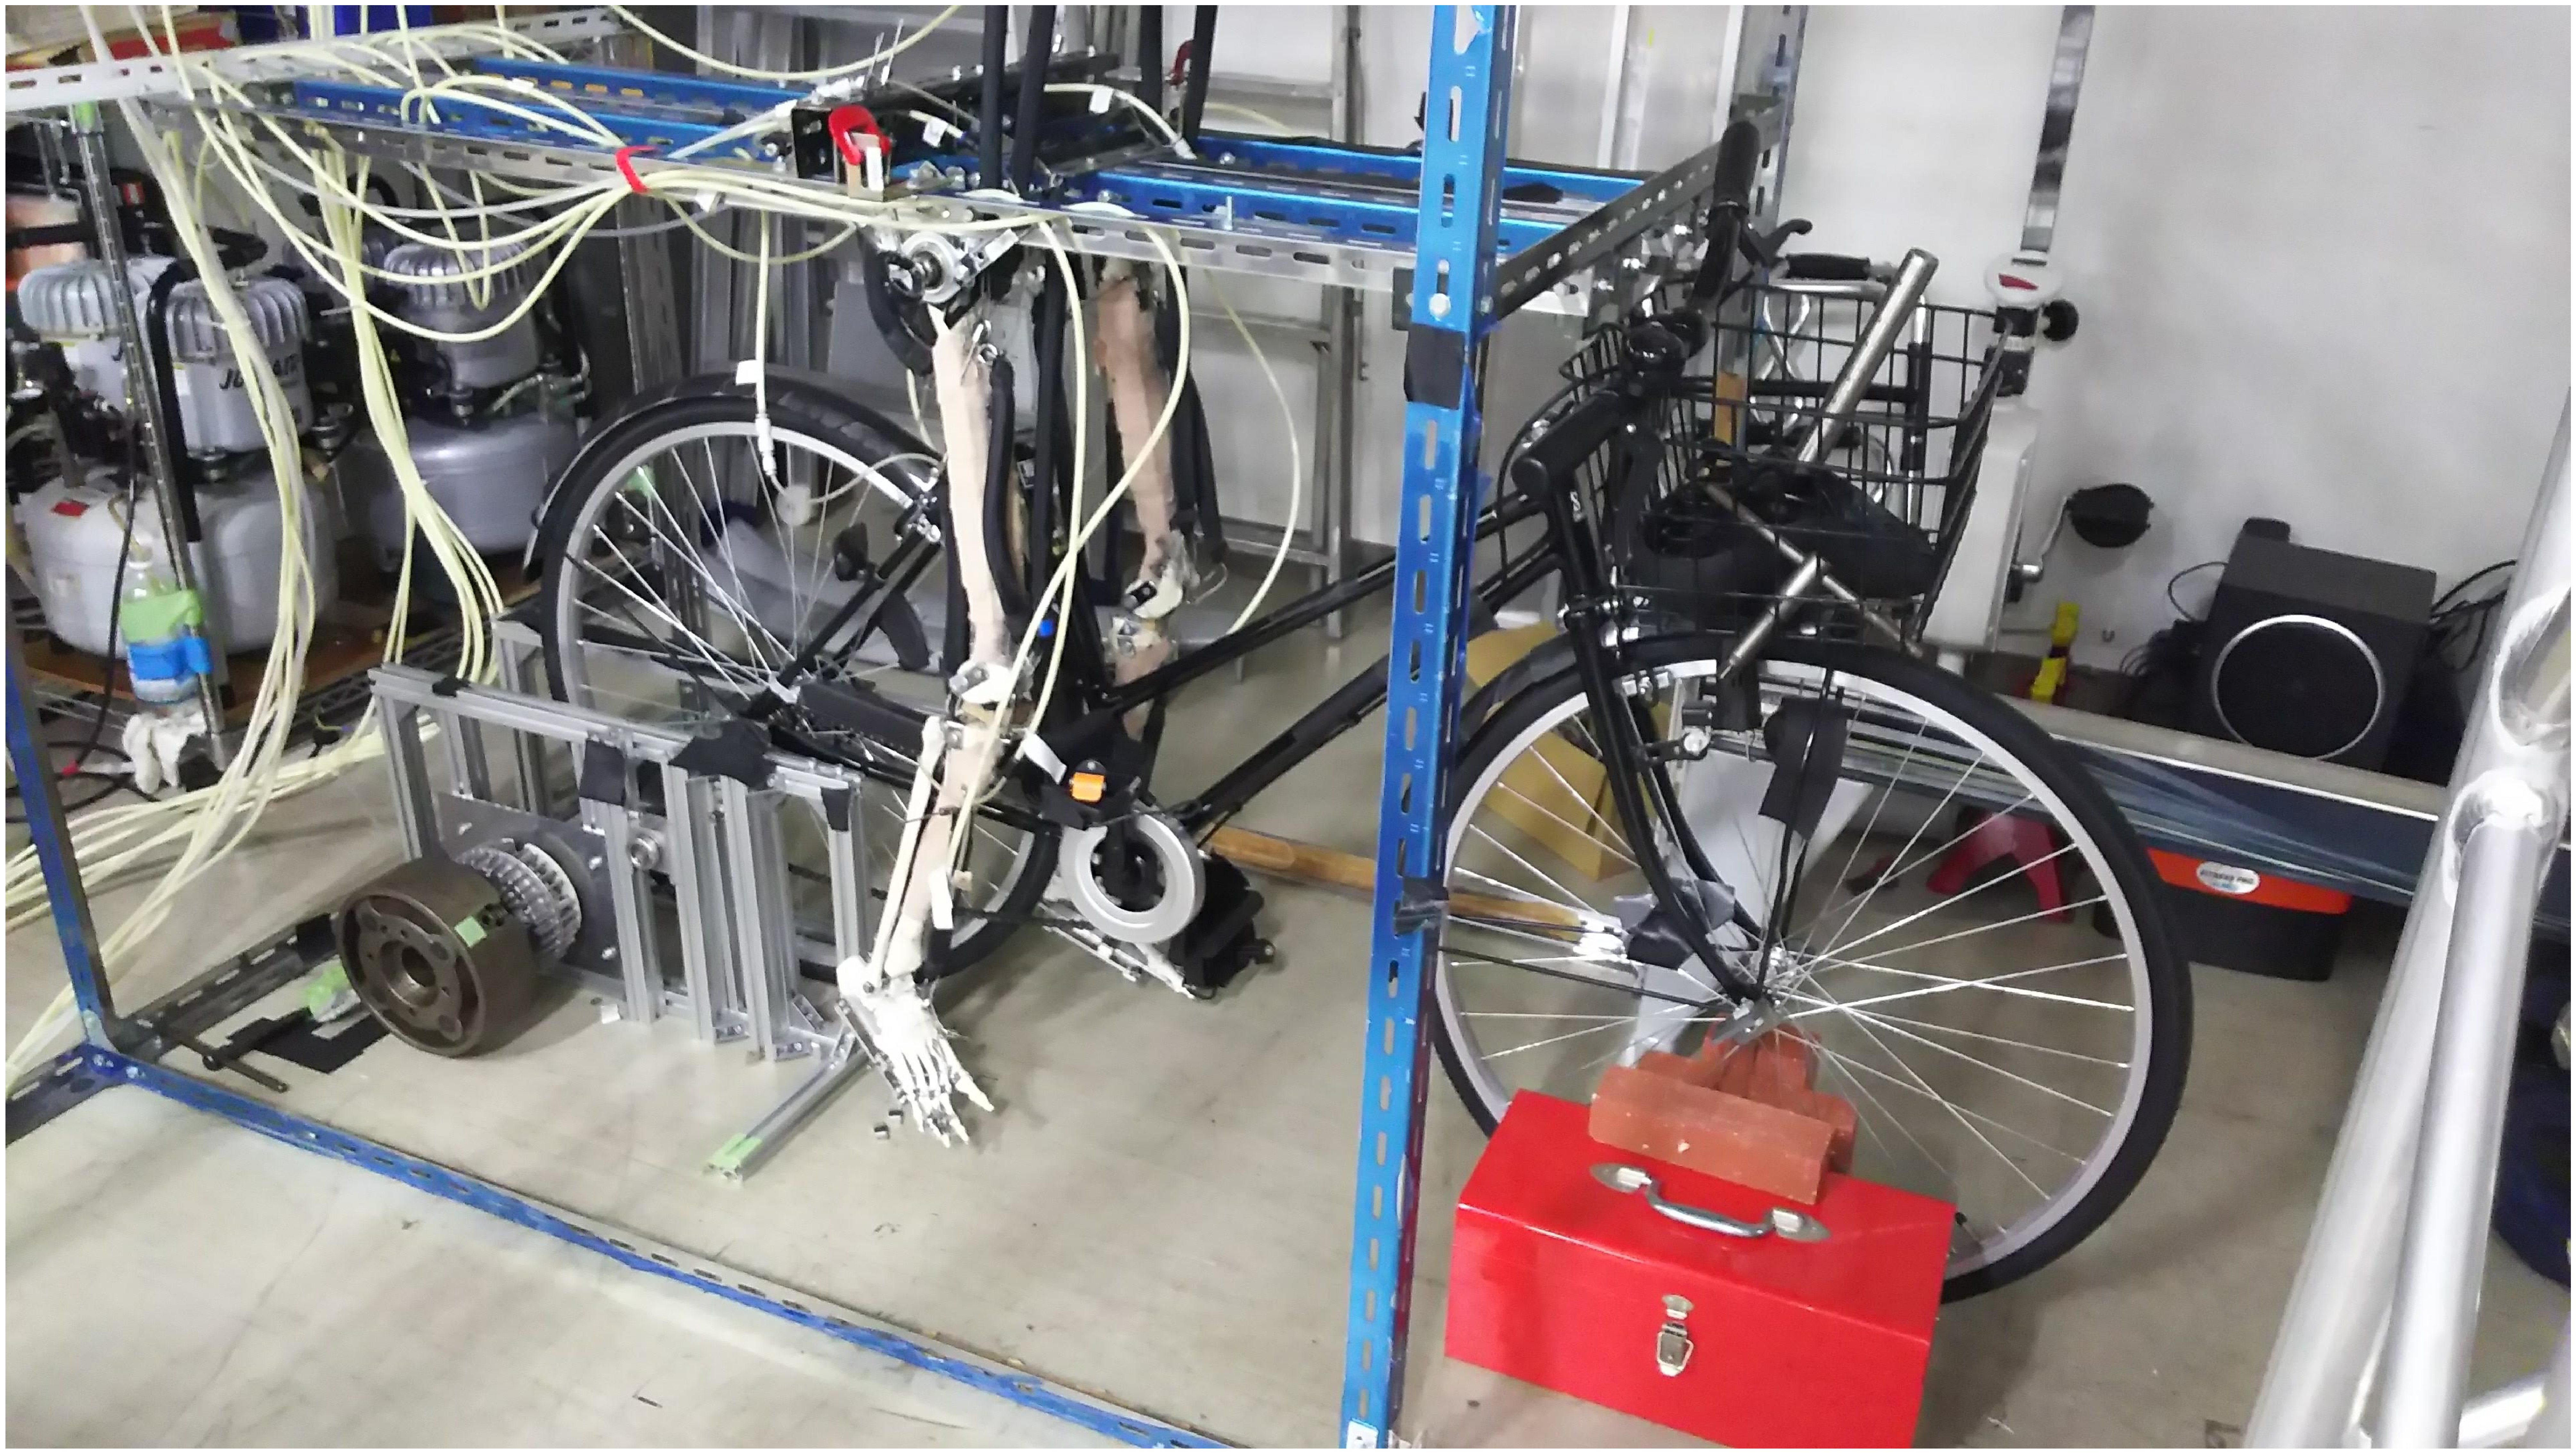
\includegraphics[width=0.75\columnwidth,clip]{Photo/BackGround/1st.eps}
  \caption{ペダリングロボット(初号機)}
  \label{初号機}
  \end{center}
\end{figure}

%TODO:2号機のお話を書く
%TODO:2号機関連の研究のリファレンスを貼る
また,先述の初号機を元にして腰を固定していない状態の二足歩行型ロボット(2号機)も製作された.こちらは先述のロボットと異なり腰が固定されておらず,二足歩行可能な形となっている.一方で関節動作に関しては先述のロボットと同様の形となっており,股関節,膝関節,足首関節それぞれがピッチ方向にのみ自由度を持っており2次元平面上における動作を再現することが出来た.先述のロボットと同様に,筋シナジーベクトルを利用し片麻痺患者と健常者の歩行の比較をロボット上で行った.
\begin{figure}[h]
  \begin{center}
  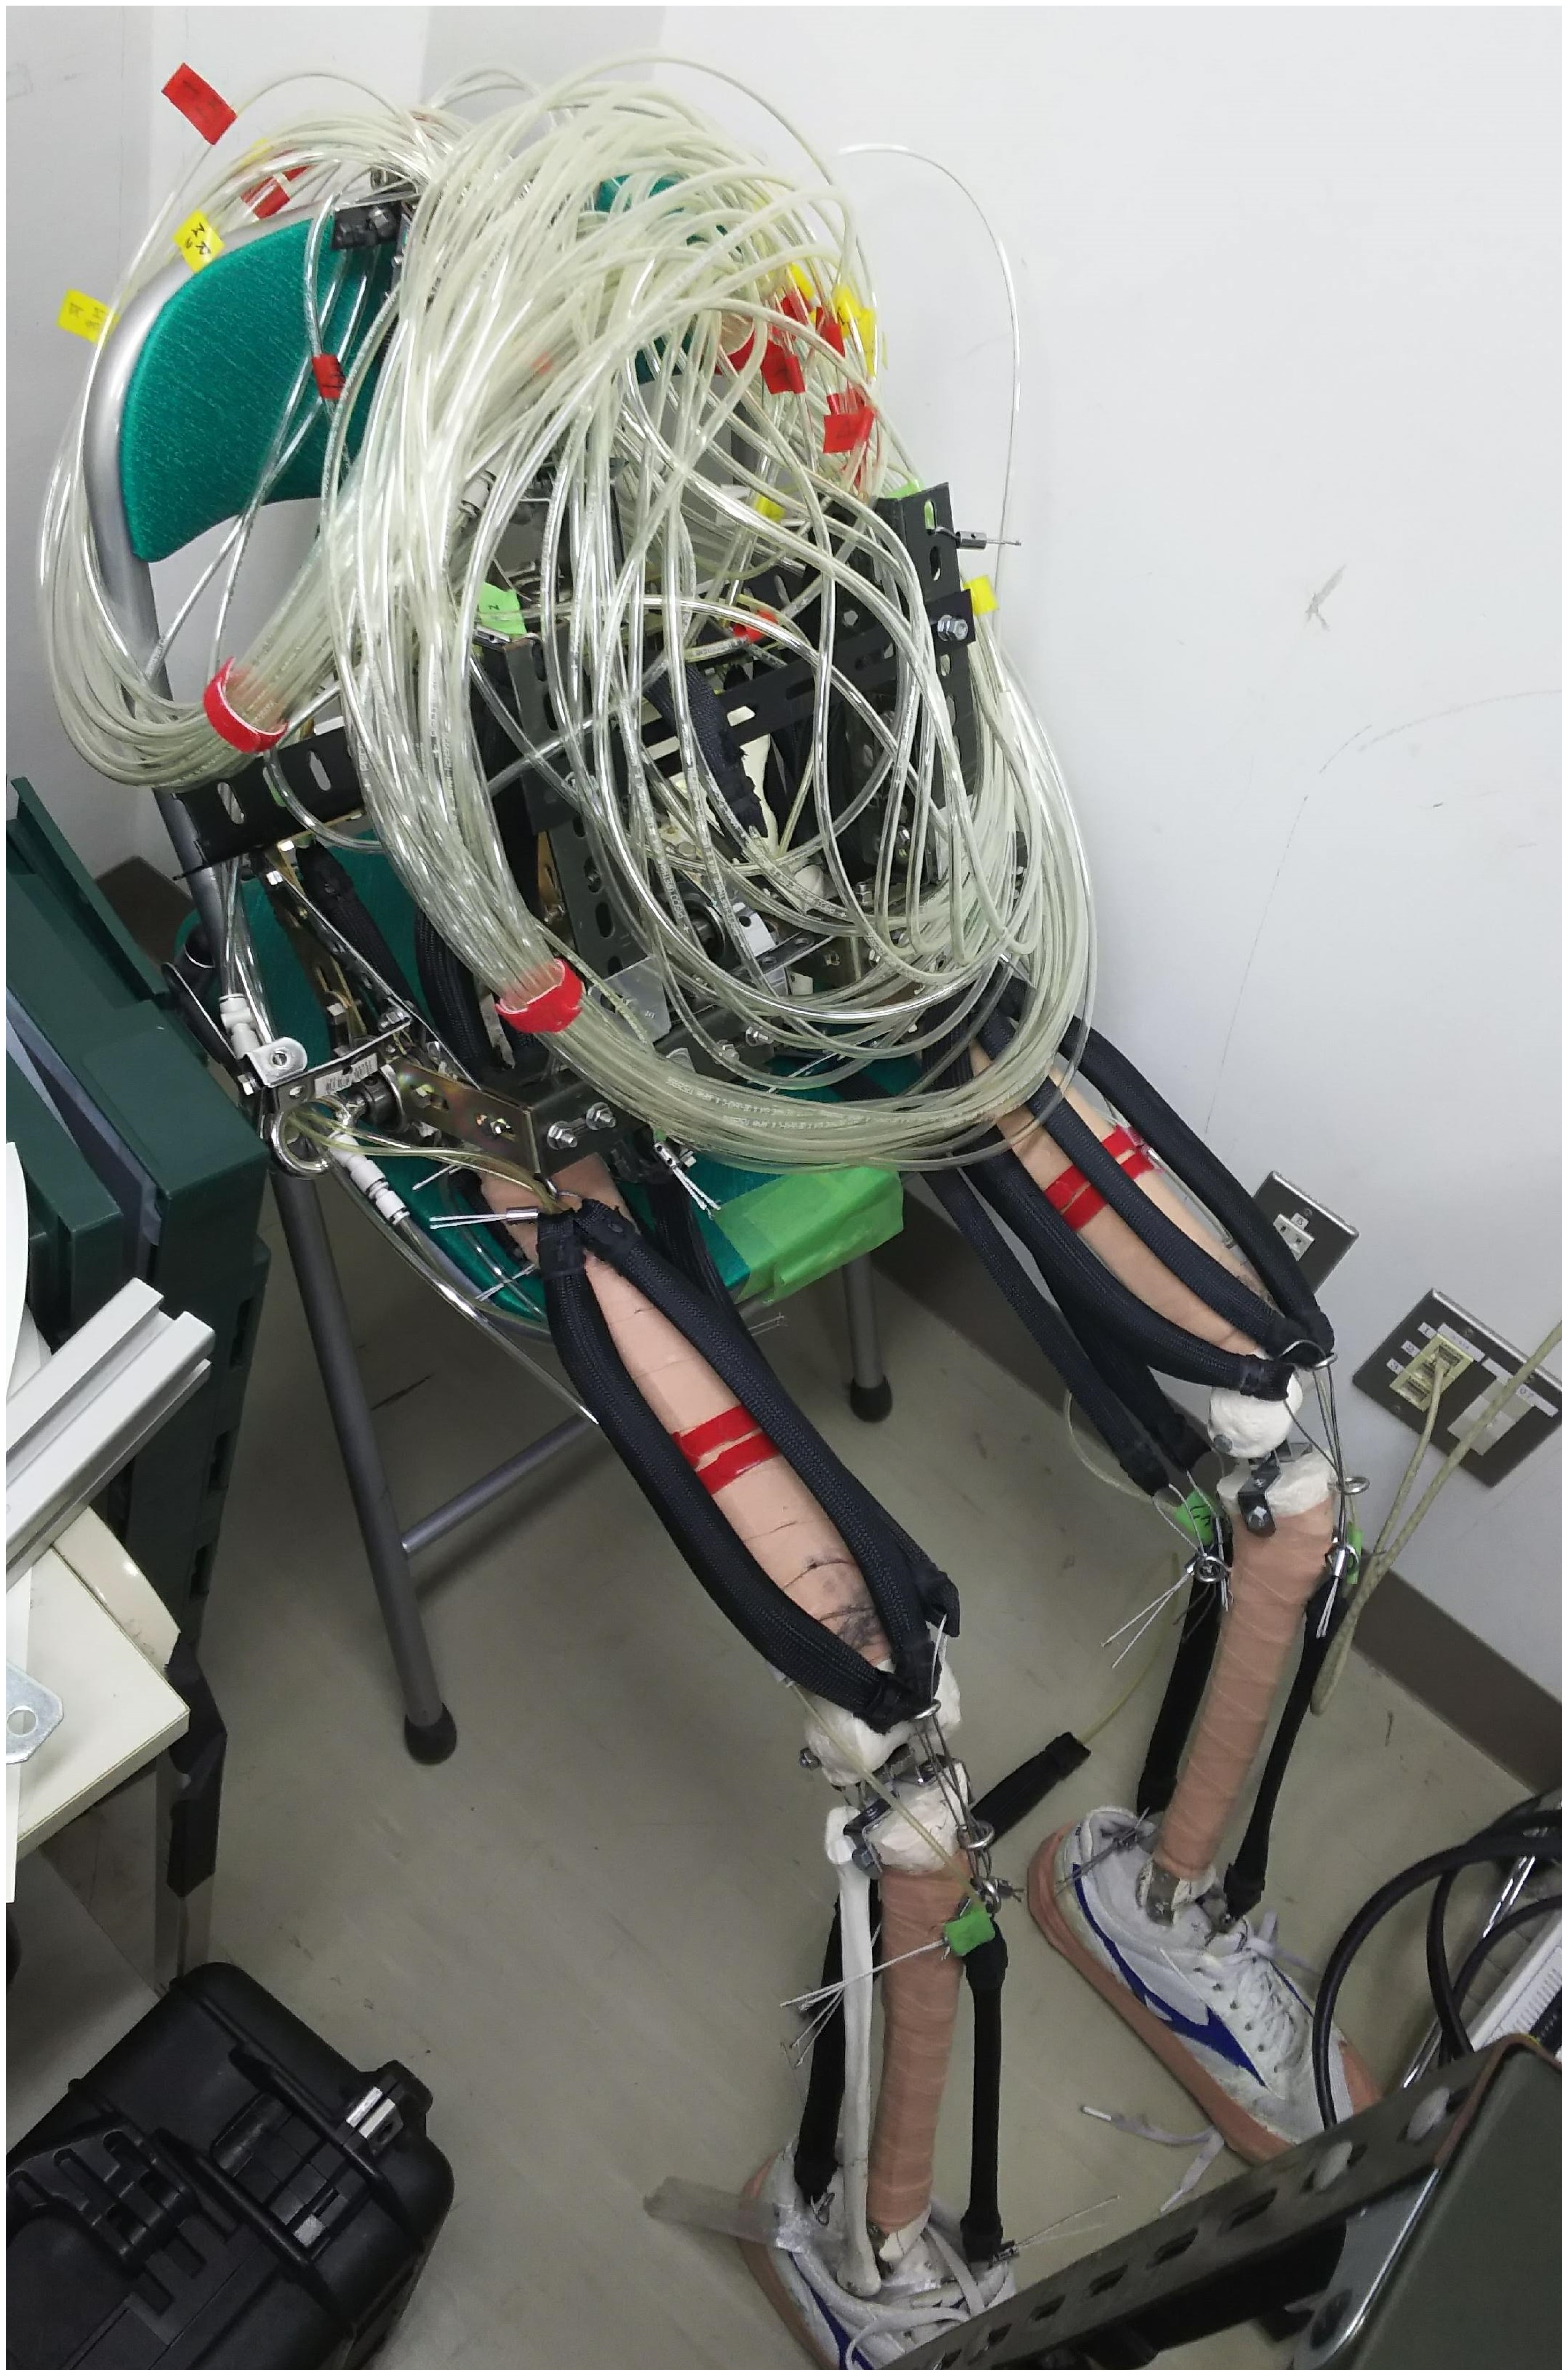
\includegraphics[width=0.5\columnwidth,clip]{Photo/BackGround/2nd.eps}
  \caption{二足歩行ロボット(2号機)}
  \label{2号機}
 \end{center}
\end{figure}

%TODO:3号機のお話を書く
これら,ペダリングロボット(初号機),2足歩行ロボット(2号機)の経験を踏まえ,今回新たに2足歩行ロボット(3号機)の開発を行った.従来の2足歩行ロボットでは自由度の制約が大きく,2次元平面上のみでの動作となっていたものが3次元空間上で動かせるものとした.

股関節部分の自由度

足関節の自由度が従来の2足歩行ロボット(2号機)ではピッチ方向の1自由度であった。一方で実際の人間の自由度はこれに加えてロール方向,ヨー方向も存在し3自由度である.

%TODO:これらを統合し,筋肉の伸長を巻き込んだシステムの話をする
今回開発を行った導電性布,シリコンを用いた伸縮センサを空気圧人工筋に組み合わせ